\chapter{Methodology}
\setcounter{secnumdepth}{3}

\paragraph{}
In this section, we describe our methodology for estimating behaviors of users in social media sites from observational data. According to the literature review, we noticed that interest and engagement are two crucial metrics for social media. These two values are dependent on many parameters, which are not easy to determine. The user and the platform (Facebook, Twitter...) are the two main sources of variation. From the user perspective, mood, stress and age \cite{f_youth_engagement} are factors modifying the two metrics. From the service side, the factors are well known from the companies, as many engineers focus on developing better solutions for the user. These solutions take into consideration the content, display, meta-data and are today more accurate due to Big Data.(ie: New EdgeRank version is taking in consideration more than 100.000 weight \cite{f_EdgeRank2}).\\
Taking into consideration the three main reasons previously mentioned - privacy, content, and technique - we decided to base our experiment on Twitter. This way, the content is normalized and the user is familiar with it because we embed the tweet: the design of each tweet is similar to the one on Twitter. In order to add fun, we picked the Tinder concept of binary classifications of girls and applied it to the tweets. This approach helped us to design a protocol based on tweets classification, which differentiates the user interest and engagement.
First of all, we give an overview of the methodology, explaining the test that we ran and the metrics used. Then, we introduce our Twitter dataset, composed of embedded tweets from user timelines. Finally, we delve into the process itself.

\section{Big picture}

\paragraph{}
In order to measure our users' behaviors, we decided to run A/B testing with two different B tests. This allows us to compare our dependent variables which are the number of likes and the time spent on a tweet. To be sure that we only keep in consideration the two dependent variables, a simple graphical design is used. This design is exactly like a PowerPoint document, where the content of each slide is an embedded tweet. The user has to decide for each slide, if the user likes or dislikes a tweet by pressing one of two different keys on the keyboard. Based on the design of Figure \ref{fig:a_b_diagram}, we create an A/B test with one initial experiment called "Calibration" (test A) and two others recording input the time (test-time-B) and the numbers of likes (test-like-B). Because of the unique design, we will explain how we select the tweets for the calibration part and the two other tests.

\begin{figure}[h]
\centering 
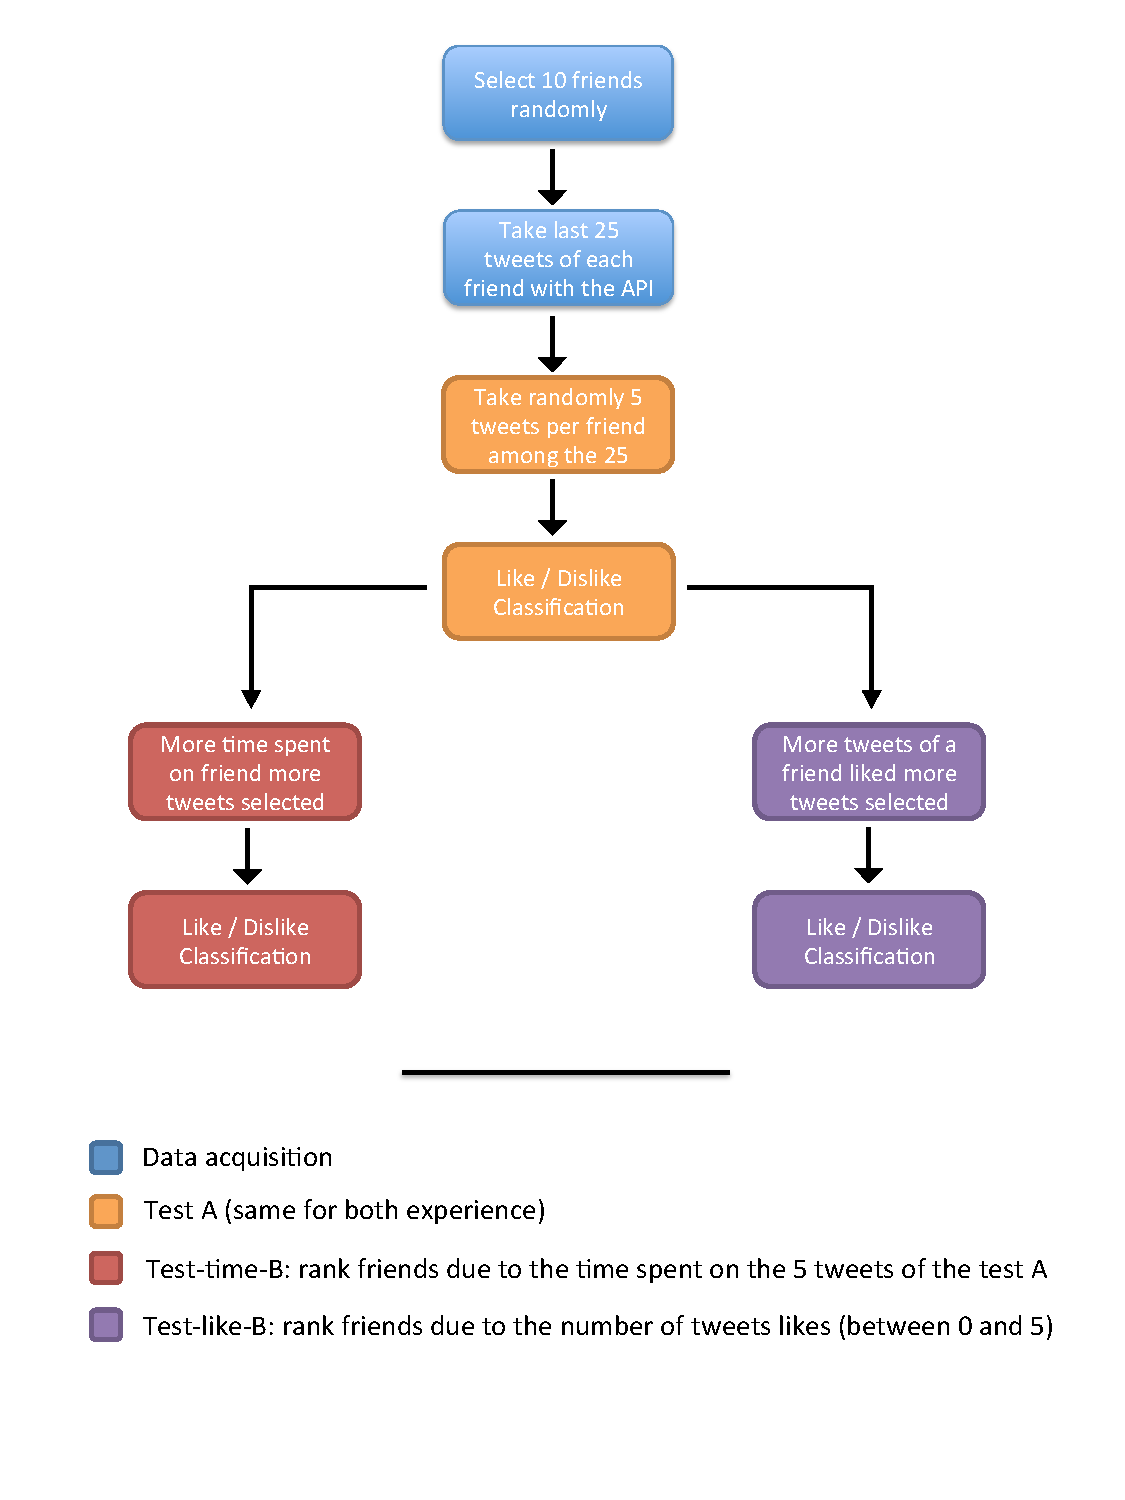
\includegraphics[width=1\columnwidth]{method/diagram} 
\caption[A/B test design]{The diagram shows the design of the A/B test. First, each user took the unique test A. After a short break of one minuit, half of the users did test-time-B. The rest of them did test-like-B.}
\label{fig:a_b_diagram} 
\end{figure}


\section{Dataset}

\paragraph{}
As mentioned before, we decided to do a binary classification (like / dislike) of the tweets coming from the user's timeline. Because we use tweets from the timeline, it is assumed that users are interested by the content to a certain extent: they follow the writer of the tweet. In order to reduce external factors, we limit the timeline to a group of 10 people the person follows, called "friends". We select 10 friends randomly who published at least 25 tweets. Thanks to this data, we create a simple timeline that we suppose is similar to the real one. When a user logs in to Twinder, we retrieve in total 250 tweets: 25 tweets coming from 10 different friends. In order to keep the timeline chronological, we select the 25 most recent tweets from each user. \\
In the motivation chapter, we said in the table \ref{tab:table_analysis} that the content of twitter is standardized with a maximum of 140 characters. However, the content can take several forms, like photos, videos, text and it starts to become more difficult to differentiate each case. We finally consider them similar to a pure text because the majority of the tweets with images contain text. After having considered the content of the tweets, the next problem that we faced was the layout of each tweet. Indeed, after displaying only the text of the tweets, we realized that the embed layout was something important for the user. It allow the person to contextualize the information and link it to twitter. (img difference of embed not). \\
The methodology of the experiment is based on the dataset assumption that we enumerated previously. The A/B test will be explained, it is composed of the test A (calibration) and the test B1 or B2.  

\section{A/B Test}

\paragraph{}
In this section, we explain the methodology of the experiment which is designed like an A/B test. We describe the two steps of the test and try to show why we chose this method to evaluate the two different behaviours of the user, which are interest and engagement.

\subsection{Test A : the calibration }

\paragraph{}
This step is common to every candidate, it is the base of our data collection and it gives us the input for the next step of the experiment. From the 250 tweets coming from 10 differents friends, we create a subset of 50 tweets. To compose this subset, we take 5 tweets randomly from each friend. By doing it this way, for the calibration test we have: 5 tweets times 10 friends which is a total of 50 tweets. Thanks to this design, the candidate is going to classify 50 tweets and then allow us to rank the interest and the engagement of the user for each one of these 10 friends.\\
Twinder, the slides application, saves each decision of the user in an object. These logs are used afterwards to define the next distribution of tweets. Mainly, the object stores: a timestamp, the decision (like / dislike), the tweet\_id and the friend\_id. This structure give us two important pieces of data: the time and the decision. After the test A, we can already display two graphs. \\
The first one is the sum of the time spent on tweets of a particular friend. Despite a tweet having a maximum length of 140 characters, we decided to normalized the time spent on a tweet per its number of characters.\\
The second one is the number of likes that a friend received. As we display 5 tweets per friends, the number of likes is between 0 and 5.\\
Thanks to these two different parameters, we are going to generate a series of 50 other tweets with two different distributions. In order to measure the user's behaviors, the distribution of the 50 tweets is going to depend on the time for test B1 and the number of likes for test B2.\\


\subsection{Tests B}

\paragraph{}
As we mentioned previously, test B depends on two different parameters: the time spent on the tweets and the number of likes. In this way, the same number of users is going to participate in test A/B1 and A/B2. We are going to describe the two implementations and explain how they are measuring the engagement and the interest.

\subsubsection{Test-time-B}

\paragraph{}
After the calibration series is completed by the user, we can obtain from the data: the number of likes per friend and the time that a user spent on a specific friend. For the test B1 we chose to use the time and then measure the engagement. As we saw in the reviewed literature, it is impossible to give a unique definition of engagement. It is driven by the action that the user can do in the platform: click, scroll, like, retweet. As we cannot identify precisely what the impacts of each action are, we decided to only take engaged time into consideration. In this way, the more time a user is spending on a friend, the more engaged he is engaged by him no, matter what he decided. The interest of the user does not have any importance. \\
As was explained previously, we are going to generate the second series of 50 tweets based on the engaged time per friend. We are going to rank the friends as a function of the engaged time, and attribute more importance to the longest time. Indeed, our goal is to increase the engaged time. \\
To generate this vector of 50 tweets, first , we retrieve from the database, the 25 tweets per friend and remove the 5 tweets used in the test A. Then we use a linear function which takes the time as input, and an integer between 1 and 20 is the output. This integer is the number of tweets that we have to take for a given friend. In this way, we are going to take 20 tweets from the friend with the maximum time spent and only 1 from the friend with the minimum time. The tweets are always selected randomly.\\
Once we have taken the tweets proportionally, we obtain a subset of more than 50 tweets coming from the 10 friends. Randomly, we will take 50 tweets from this subset, this method leaves the possibility of every friend appearing in the next series. After this, we repeat the classification experiment like in test A and take the logs of the decision.\\
This method is designed to increase the engaged time, we only take into consideration the time spent on friends in series A when creating the next subset of 50 tweets. Doing this, we suppose that the time spent on the second series is going to increase. While this method is supposed to increase the engaged time, the second method considers the interest of the users.


\subsubsection{Test-Like-B}

\paragraph{}
While test B1 focuses on the engagement,test B2 only considers the interest of the user. The interest of users is like the engagement, something not easy to measure, especially if we consider the two main ways which we can show it: retweet and mark as favorite. Thanks to the simple design of our application, we simplify the concept and allow the user to only choose if he likes or dislikes it. Of course, it is simplistic to measure the interest in a binary way but if we do the parallel with Tinder, it creates a good approximation as the user has to make a decision to pass to the next tweet. \\
Exactly like the previous test B1, we are going to select a subset of 50 tweets based on the number of likes received per user. Then, we use the same linear function except the  which take in input the number of tweets liked per friend an output a number between 1 and 20. If a user likes the 5 tweets of a given friend in test A, then we take 20 tweets from that friend in subset. Every time, we randomly select the tweet for a given friend. After applying the same process for each friend, we take 50 random tweets from the subset, which become our input for test B2. The user has to pass the classification test again, and we record the logs of the new series. \\
The B1 and B2 tests were designed to isolate two different metrics: time engaged and interest. We submitted test A to every candidate and had half of the candidates do test B1 and the other half, test B2. In order to better describe the experiment, the next chapter explains the experimental settings.